\pdfminorversion=6 % this is needed to be able to include pdf 1.6. 
                    % For some reasons some old HPSG proceedings have pdf 1.6
\documentclass[11pt,a4paper,fleqn]{article}
\usepackage{times}
\thispagestyle{empty}



\usepackage[T1]{fontenc}   % Silbentrennung

\usepackage[utf8x]{inputenc}
                                                                                                                             
\hyphenation{Acad-e-my}

\usepackage[bookmarks=true,bookmarksopen=true,%
breaklinks=true,%
draft=false,plainpages=false,hyperfootnotes=false,%
pdfauthor={Stefan  Müller, Anke Holler (Editors)},%
pdftitle={Proceedings of the 27th International Conference on Head-Driven Phrase Structure Grammar},%
pdfkeywords={HPSG}%,
pdftex=true%
%ps2pdf=true  %ohne diesen Treiber geht der Zeilenumbruch in URLs
]{hyperref}% for pdf files
\hypersetup{colorlinks=false, pdfborder={0 0 0}}

\usepackage{pdfpages}
\pdfinclusioncopyfonts=1

\newcommand\formatauthor[2]{\begin{tabular}[t]{@{}c@{}}
  {\LARGE#1\strut}\\
  {\small#2\strut}\\
  \rule{\dimexpr0.5\linewidth-1em}{0pt}
  \end{tabular}\xhfill\ignorespaces}
\newcommand\xhfill{\hspace{1em plus 1fill}}

\begin{document}

\begin{center}
{\Large
                {\bfseries Proceedings of the 27th International Conference on\par Head-Driven Phrase Structure Grammar\par}

                \vspace{8ex}

                     Online (Berlin/Seattle)\\[\baselineskip]

                        Stefan  M{\"u}ller, Anke Holler (Editors)\\[\baselineskip]

                                2020\\[\baselineskip]

                          CSLI Publications\\[\baselineskip]

              http://csli-publications.stanford.edu/HPSG/2020 \\[4\baselineskip]

The papers are published under a \href{http://creativecommons.org/licenses/by/4.0/}{CC-BY license}:\\[3pt]
\href{http://creativecommons.org/licenses/by/4.0/}{http://creativecommons.org/licenses/by/4.0/}
}
\end{center}
\newpage
\tableofcontents

\newpage

\section*{Editor's note}
\addcontentsline{toc}{section}{Editor's note}
%% -*- coding:utf-8 -*-
The 27th International Conference on Head-Driven Phrase Structure Grammar (2020) was planned to take
place in Leuven (organized by Frank Van Eynde and Liesbeth Augustinus), but due to the Corona
pandemic it was organized online by Stefan Müller (Humboldt Universität zu Berlin) and Olga
Zamaraeva (University of Washington, Seattle).


The conference featured 3 invited talks and 11 papers selected by the program committee 
(Anne Abeillé, 
    Doug Arnold,
    Emily Bender,
    Felix Bildhauer,
    Hans Boas,
    Olivier Bonami,
    Francis Bond, 
    Gosse Bouma, 
    Antonio Branco, 
    Rui Chaves, 
    Philippa Cook, 
    Berthold Crysmann,
    Dan Flickinger, 
    Antske Fokkens, 
    Petter Haugereid, 
    Fabiola Henri, 
    Thomas Hoffmann, 
    Anke Holler (chair),
    Gianina Iordăchioaia,
    Paul Kay, 
    Jong-Bok Kim, 
    Jean-Pierre Koenig, 
    David Lahm, 
    Bob Levine, 
    Nurit Melnik, 
    Laura Michaelis, 
    Philip Miller, 
    Stefan Müller, 
    Tsuneko Nakazawa, 
    Petya Osenova, 
    Rainer Osswald, 
    Gerald Penn, 
    Frank Richter, 
    Louisa Sadler, 
    Manfred Sailer, 
    Pollet Samvellian, 
    Jesse Tseng, 
    Stephen Wechsler, 
    Eun-Jung Yoo, 
    Shûichi Yatabe).


% wie viele?
%In total there were x  submissions to the conference and x submissions to the workshop.
We want to thank the program committee for putting this nice program together.

% Thanks go to Gabriela Bîlbîie and Emil Ionescu, who were in charge of local
% arrangements.
 

As in the past years the contributions to the conference proceedings are based on the five page abstract
that was reviewed by the %respective 
program committee, but there is no additional reviewing of the
longer contribution to the proceedings. To ensure easy access and fast publication we have chosen an electronic format.

The proceedings include all the papers of the conference except the ones by Liesbeth Augustinus, Gosse Bouma, Frank Van
Eynde \& Jong-Bok Kim, Gert Webelhuth and Shûichi Yatabe.


\newpage
        \setcounter{page}{5}
        \phantomsection
        \addcontentsline{toc}{section}{Gabriel Aguila-Multner, Berthold Crysmann: An inside-out approach to
French causatives}
\thispagestyle{empty}

\begin{center}
  {\huge\bfseries An inside-out approach to
French causatives\par}

  \bigskip

~\\
\begingroup
\setlength{\leftskip}{0pt plus 1fill}
\setlength{\rightskip}{0pt plus 1fill}
\setlength{\parindent}{0pt}
\setlength{\parfillskip}{0pt}
  \formatauthor{Gabriel Aguila-Multner}{\begin{tabular}{@{}c@{}}Université de Paris,
Laboratoire de linguistique formelle, CNRS\end{tabular}}
\formatauthor{Berthold Crysmann}{\begin{tabular}{@{}c@{}}Université de Paris,
Laboratoire de linguistique formelle, CNRS\end{tabular}}

\par\endgroup

  \vspace*{8ex}

  Proceedings of the 27th International Conference on\par Head-Driven Phrase Structure Grammar

  \bigskip

  Online (Berlin/Seattle)

  \medskip

  Stefan  Müller, Anke Holler (Editors)

  \medskip

  2020

  \medskip

  CSLI Publications

  \medskip

  pages 5--25

  \medskip

  \url{http://csli-publications.stanford.edu/HPSG/2020}
\end{center}
\vfill

\noindent
Keywords: Clitic climbing,
French, HPSG, causative, faire, periphrasis, VP structure


\vfill
\noindent
% APA Style
Aguila-Multner, Gabriel, \& Crysmann, Berthold. 2020. An inside-out approach to
French causatives. In Müller, Stefan, \& Holler, Anke (Eds.), \emph{{Proceedings of the 27th International Conference on Head-Driven Phrase Structure Grammar, Online (Berlin/Seattle)}}, 5--25. Stanford,
CA: CSLI Publications. \hfill\href{http://creativecommons.org/licenses/by/4.0/}{
\includegraphics[height=.75em]{Includes/ccby-eps-converted-to.pdf}}

\newpage
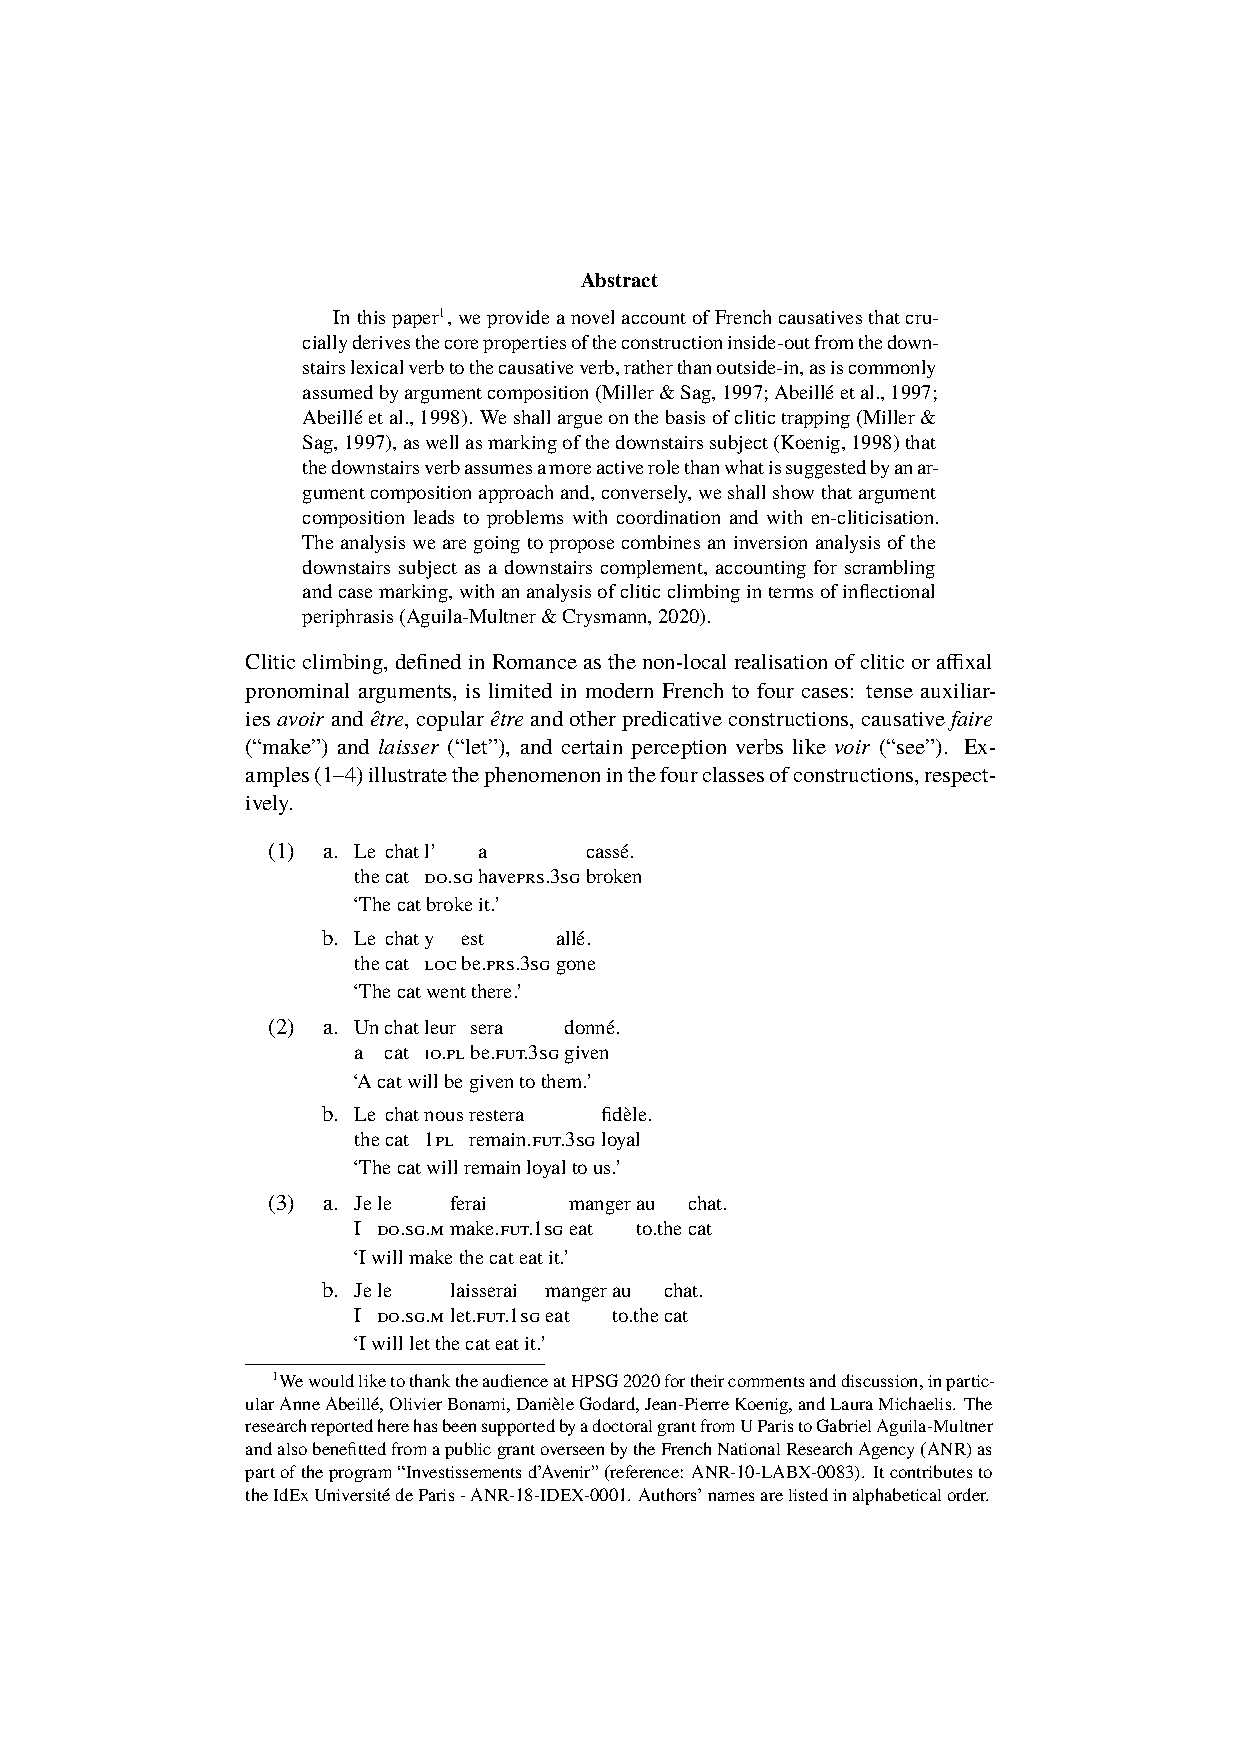
\includepdf[pages=-,pagecommand=\thispagestyle{plain}]{Includes/aguila-multner-crysmann.pdf}
        \setcounter{page}{26}
        \phantomsection
        \addcontentsline{toc}{section}{Robert D. Borsley: On a family of Welsh constructions}
\thispagestyle{empty}

\begin{center}
  {\huge\bfseries On a family of Welsh constructions\par}

  \bigskip

~\\
\begingroup
\setlength{\leftskip}{0pt plus 1fill}
\setlength{\rightskip}{0pt plus 1fill}
\setlength{\parindent}{0pt}
\setlength{\parfillskip}{0pt}
  \formatauthor{Robert D. Borsley}{\begin{tabular}{@{}c@{}}University of Essex and Bangor University\end{tabular}}

\par\endgroup

  \vspace*{8ex}

  Proceedings of the 27th International Conference on\par Head-Driven Phrase Structure Grammar

  \bigskip

  Online (Berlin/Seattle)

  \medskip

  Stefan  Müller, Anke Holler (Editors)

  \medskip

  2020

  \medskip

  CSLI Publications

  \medskip

  pages 26--46

  \medskip

  \url{http://csli-publications.stanford.edu/HPSG/2020}
\end{center}
\vfill

\noindent
Keywords: unbounded dependency constructions, wh-interrogatives, free relatives, cleft clauses, Welsh


\vfill
\noindent
% APA Style
Borsley, Robert D. 2020. On a family of Welsh constructions. In Müller, Stefan, \& Holler, Anke (Eds.), \emph{{Proceedings of the 27th International Conference on Head-Driven Phrase Structure Grammar, Online (Berlin/Seattle)}}, 26--46. Stanford,
CA: CSLI Publications. \hfill\href{http://creativecommons.org/licenses/by/4.0/}{
\includegraphics[height=.75em]{Includes/ccby-eps-converted-to.pdf}}

\newpage
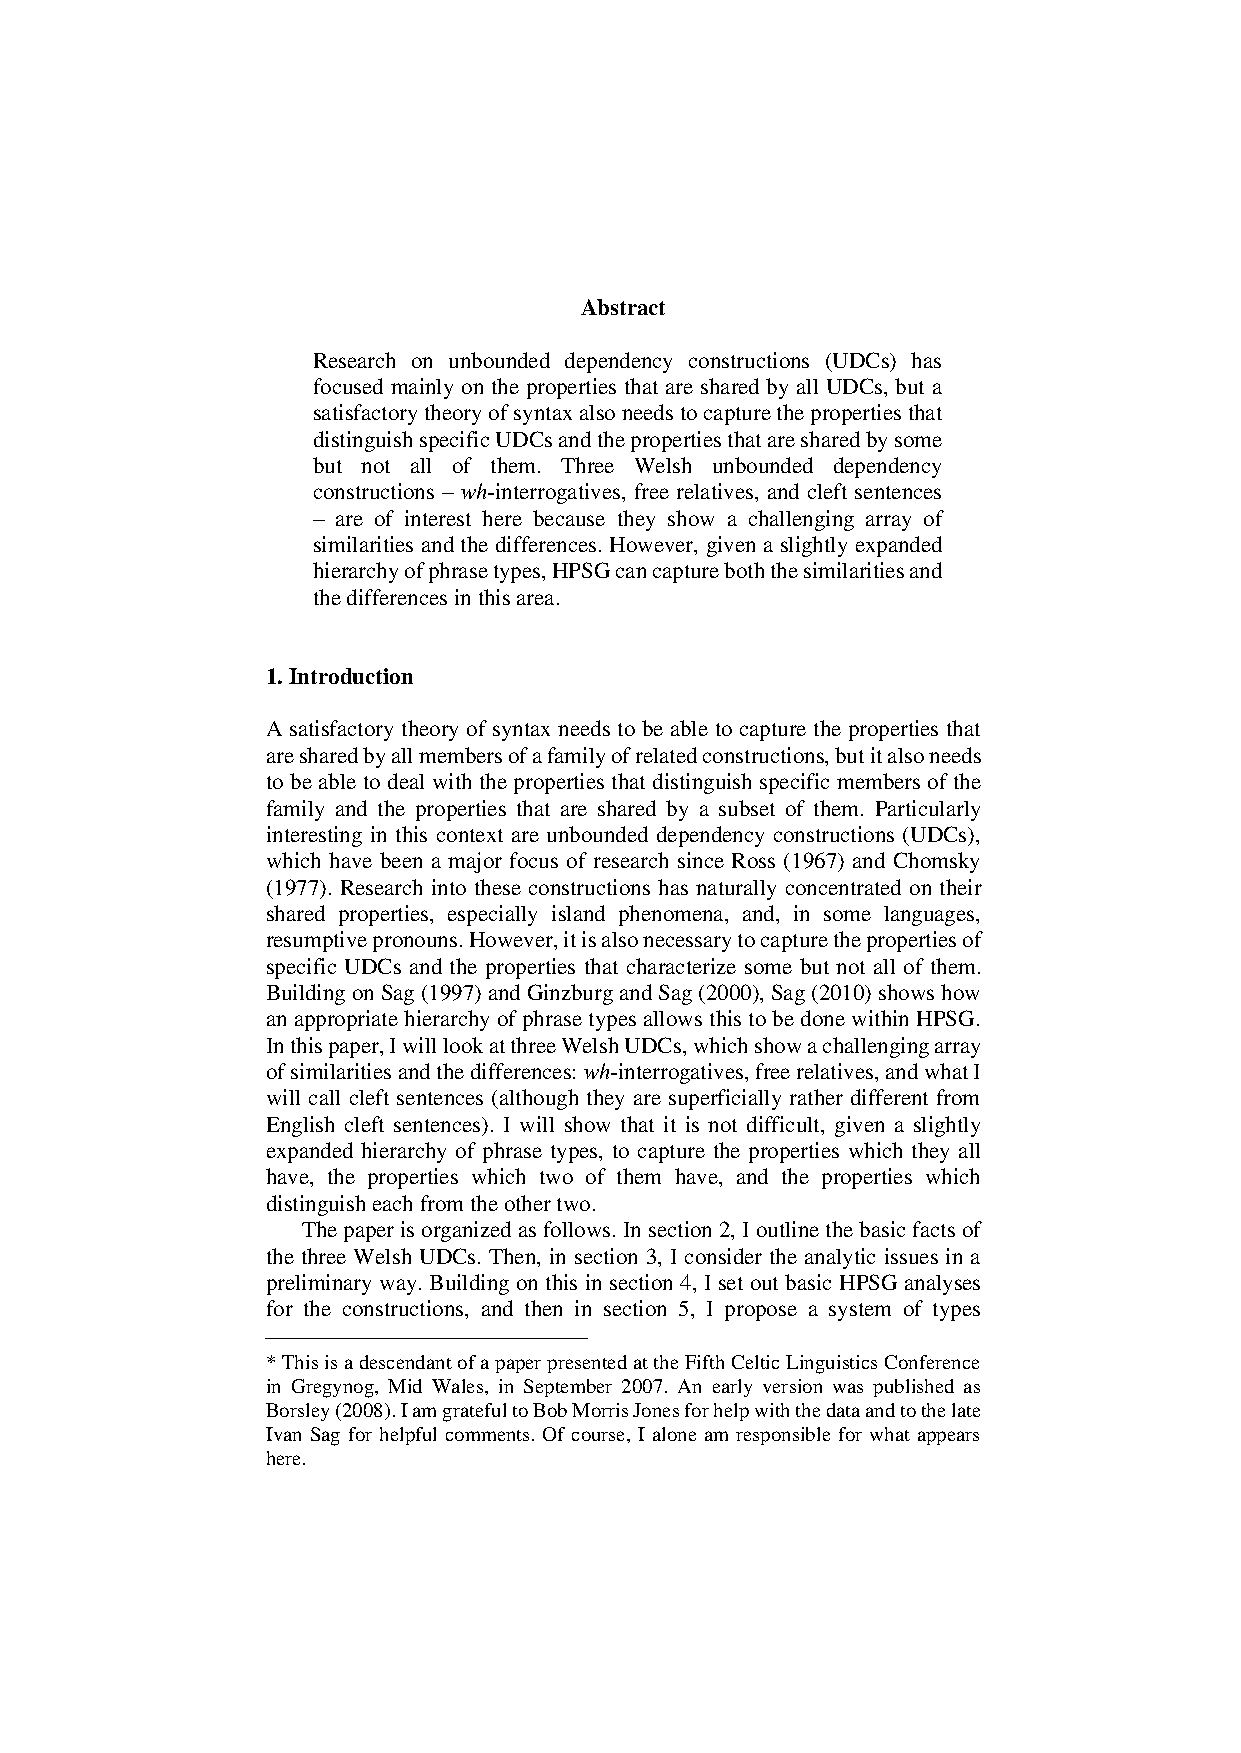
\includepdf[pages=-,pagecommand=\thispagestyle{plain}]{Includes/borsley.pdf}
        \setcounter{page}{47}
        \phantomsection
        \addcontentsline{toc}{section}{Rui P. Chaves, Paul Kay, Laura A. Michaelis: Unrealized arguments in SBCG}
\thispagestyle{empty}

\begin{center}
  {\huge\bfseries Unrealized arguments in SBCG\par}

  \bigskip

~\\
\begingroup
\setlength{\leftskip}{0pt plus 1fill}
\setlength{\rightskip}{0pt plus 1fill}
\setlength{\parindent}{0pt}
\setlength{\parfillskip}{0pt}
  \formatauthor{Rui P. Chaves}{\begin{tabular}{@{}c@{}}University at Buffalo,
SUNY\end{tabular}}
\formatauthor{Paul Kay}{\begin{tabular}{@{}c@{}}University of California, Berkeley\end{tabular}}
\formatauthor{Laura A. Michaelis}{\begin{tabular}{@{}c@{}}University of Colorado at Boulder\end{tabular}}

\par\endgroup

  \vspace*{8ex}

  Proceedings of the 27th International Conference on\par Head-Driven Phrase Structure Grammar

  \bigskip

  Online (Berlin/Seattle)

  \medskip

  Stefan  Müller, Anke Holler (Editors)

  \medskip

  2020

  \medskip

  CSLI Publications

  \medskip

  pages 47--67

  \medskip

  \url{http://csli-publications.stanford.edu/HPSG/2020}
\end{center}
\vfill

\noindent
Keywords: Sign-Based Construction
Grammar, Frames, Null Instantiation.


\vfill
\noindent
% APA Style
Chaves, Rui P., Kay, Paul, \& Michaelis, Laura A. 2020. Unrealized arguments in SBCG. In Müller, Stefan, \& Holler, Anke (Eds.), \emph{{Proceedings of the 27th International Conference on Head-Driven Phrase Structure Grammar, Online (Berlin/Seattle)}}, 47--67. Stanford,
CA: CSLI Publications. \hfill\href{http://creativecommons.org/licenses/by/4.0/}{
\includegraphics[height=.75em]{Includes/ccby-eps-converted-to.pdf}}

\newpage
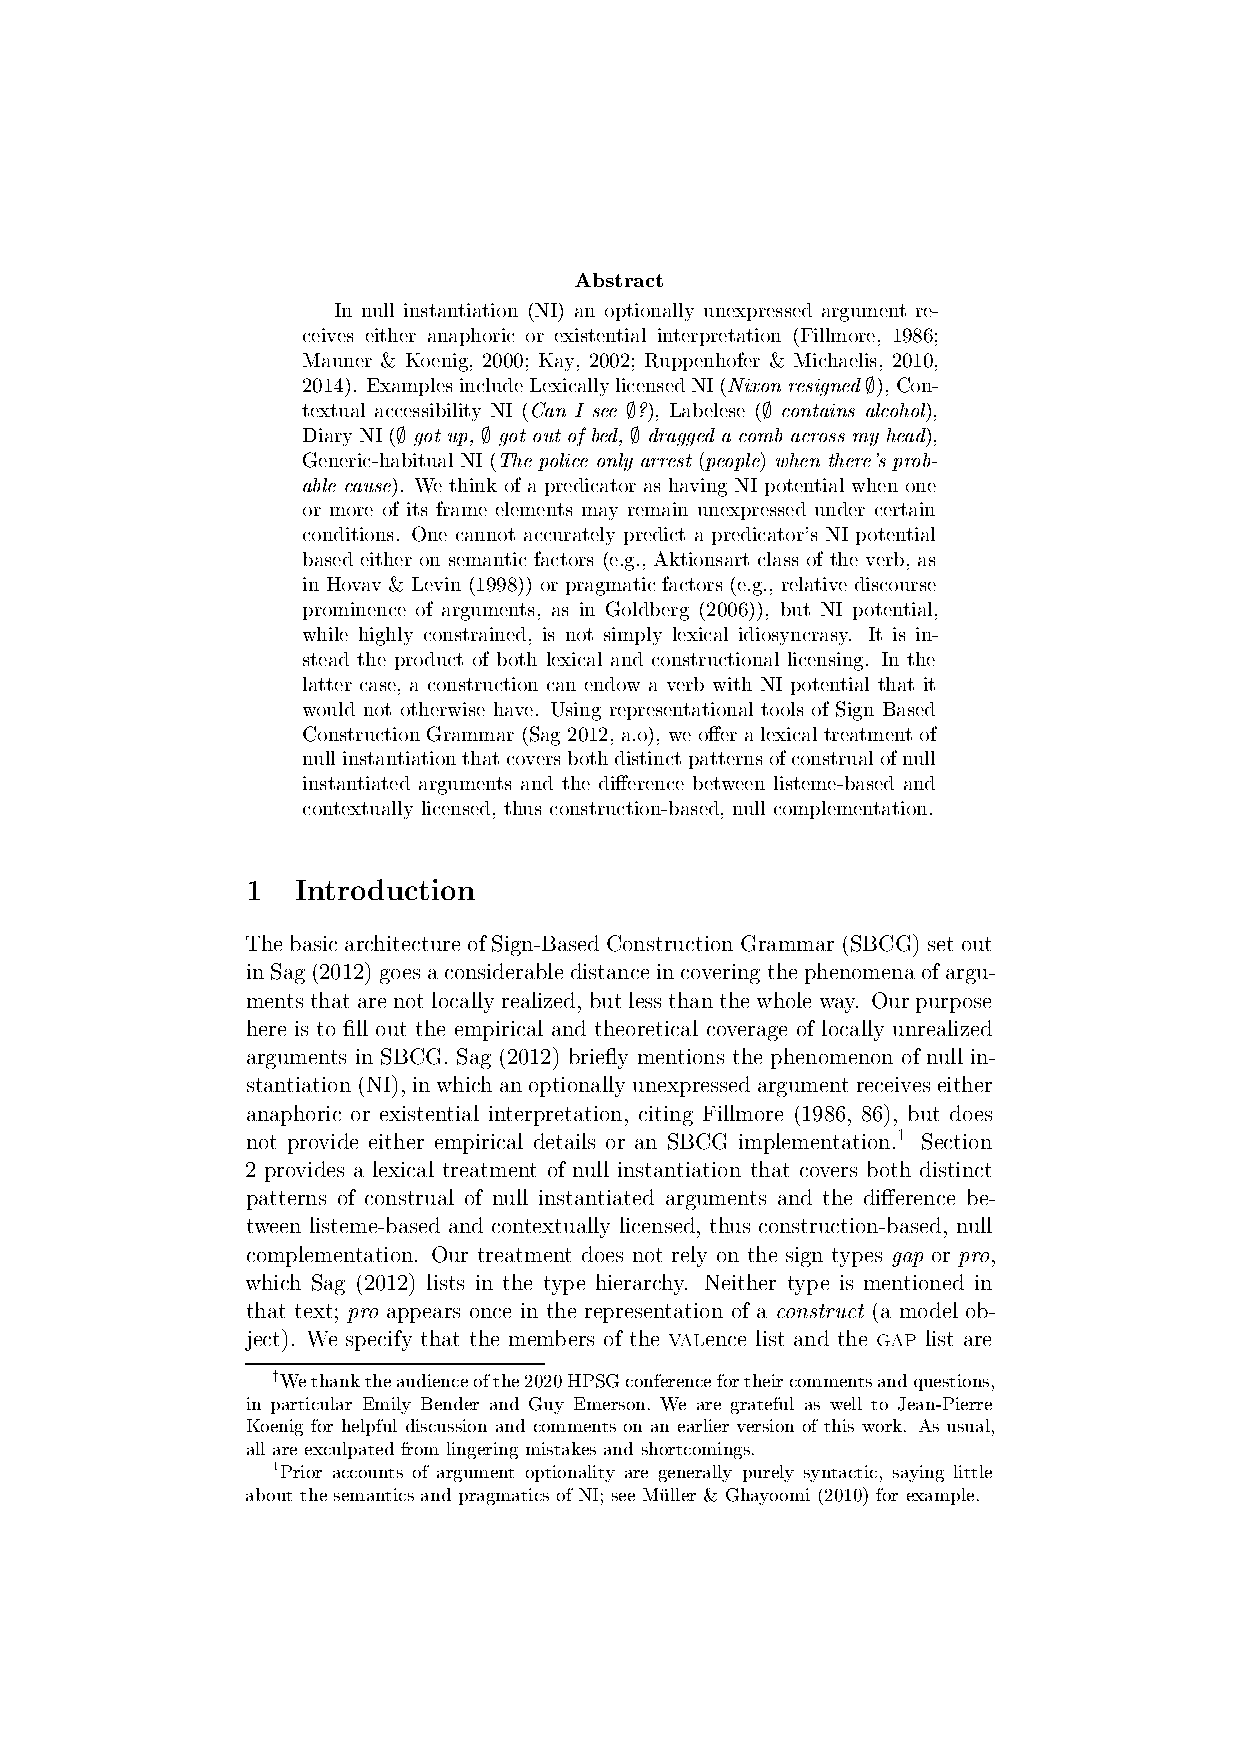
\includepdf[pages=-,pagecommand=\thispagestyle{plain}]{Includes/ckm.pdf}
        \setcounter{page}{68}
        \phantomsection
        \addcontentsline{toc}{section}{David Gyorfi: Challenges in Kazakh Auxiliary Selection}
\thispagestyle{empty}

\begin{center}
  {\huge\bfseries Challenges in Kazakh Auxiliary Selection\par}

  \bigskip

~\\
\begingroup
\setlength{\leftskip}{0pt plus 1fill}
\setlength{\rightskip}{0pt plus 1fill}
\setlength{\parindent}{0pt}
\setlength{\parfillskip}{0pt}
  \formatauthor{David Gyorfi}{\begin{tabular}{@{}c@{}}University of Surrey\end{tabular}}

\par\endgroup

  \vspace*{8ex}

  Proceedings of the 27th International Conference on\par Head-Driven Phrase Structure Grammar

  \bigskip

  Online (Berlin/Seattle)

  \medskip

  Stefan  Müller, Anke Holler (Editors)

  \medskip

  2020

  \medskip

  CSLI Publications

  \medskip

  pages 68--87

  \medskip

  \url{http://csli-publications.stanford.edu/HPSG/2020}
\end{center}
\vfill

\noindent
Keywords: HPSG, Online type construction, Kazakh, auxiliary verbs


\vfill
\noindent
% APA Style
Gyorfi, David. 2020. Challenges in Kazakh Auxiliary Selection. In Müller, Stefan, \& Holler, Anke (Eds.), \emph{{Proceedings of the 27th International Conference on Head-Driven Phrase Structure Grammar, Online (Berlin/Seattle)}}, 68--87. Stanford,
CA: CSLI Publications. \hfill\href{http://creativecommons.org/licenses/by/4.0/}{
\includegraphics[height=.75em]{Includes/ccby-eps-converted-to.pdf}}

\newpage
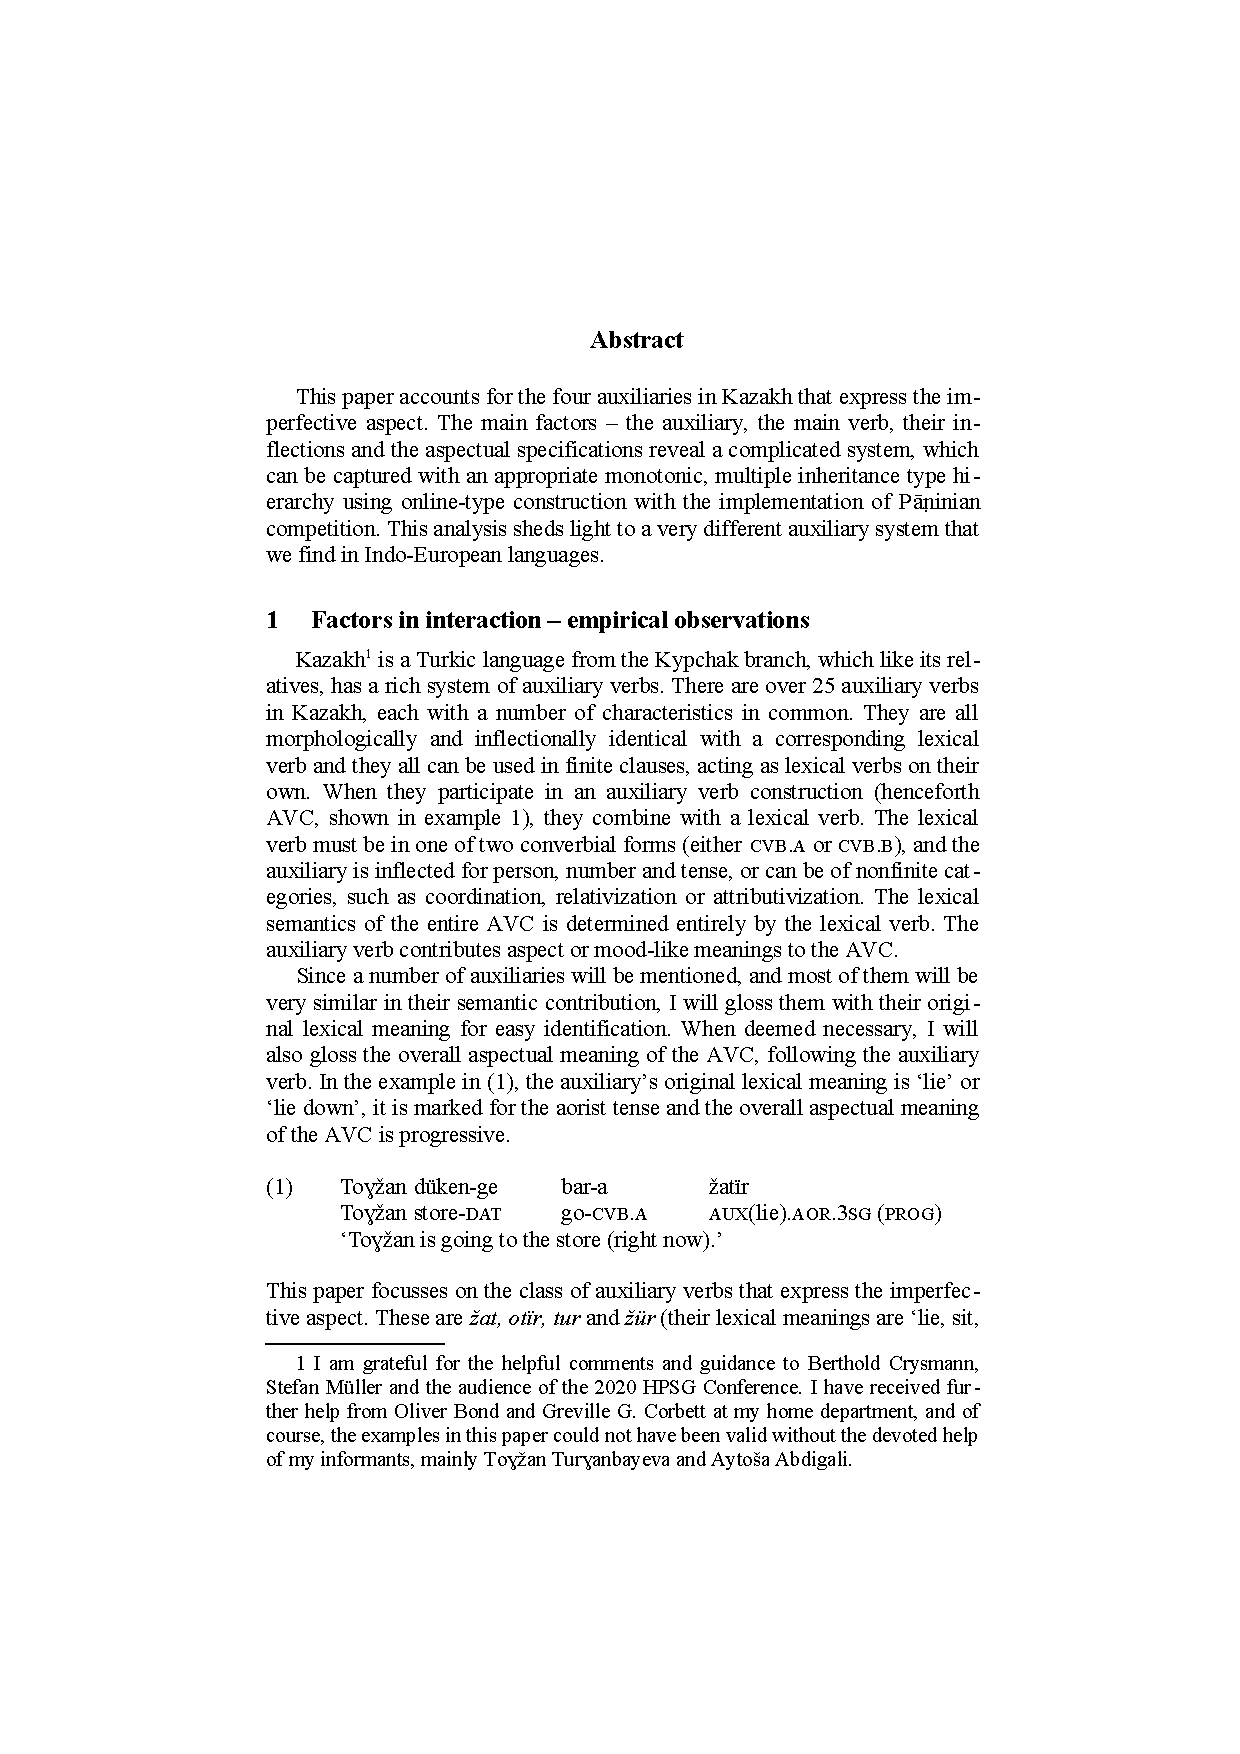
\includepdf[pages=-,pagecommand=\thispagestyle{plain}]{Includes/gyorfi.pdf}
        \setcounter{page}{88}
        \phantomsection
        \addcontentsline{toc}{section}{Petter Haugereid: An incremental approach to verb clusters in German}
\thispagestyle{empty}

\begin{center}
  {\huge\bfseries An incremental approach to verb clusters in German\par}

  \bigskip

~\\
\begingroup
\setlength{\leftskip}{0pt plus 1fill}
\setlength{\rightskip}{0pt plus 1fill}
\setlength{\parindent}{0pt}
\setlength{\parfillskip}{0pt}
  \formatauthor{Petter Haugereid}{\begin{tabular}{@{}c@{}}Western Norway University of Applied Sciences\end{tabular}}

\par\endgroup

  \vspace*{8ex}

  Proceedings of the 27th International Conference on\par Head-Driven Phrase Structure Grammar

  \bigskip

  Online (Berlin/Seattle)

  \medskip

  Stefan  Müller, Anke Holler (Editors)

  \medskip

  2020

  \medskip

  CSLI Publications

  \medskip

  pages 88--105

  \medskip

  \url{http://csli-publications.stanford.edu/HPSG/2020}
\end{center}
\vfill

\noindent
Keywords: HPSG, German, Verb Clusters, Cross-Serial Dependencies, Incremental Parsing


\vfill
\noindent
% APA Style
Haugereid, Petter. 2020. An incremental approach to verb clusters in German. In Müller, Stefan, \& Holler, Anke (Eds.), \emph{{Proceedings of the 27th International Conference on Head-Driven Phrase Structure Grammar, Online (Berlin/Seattle)}}, 88--105. Stanford,
CA: CSLI Publications. \hfill\href{http://creativecommons.org/licenses/by/4.0/}{
\includegraphics[height=.75em]{Includes/ccby-eps-converted-to.pdf}}

\newpage
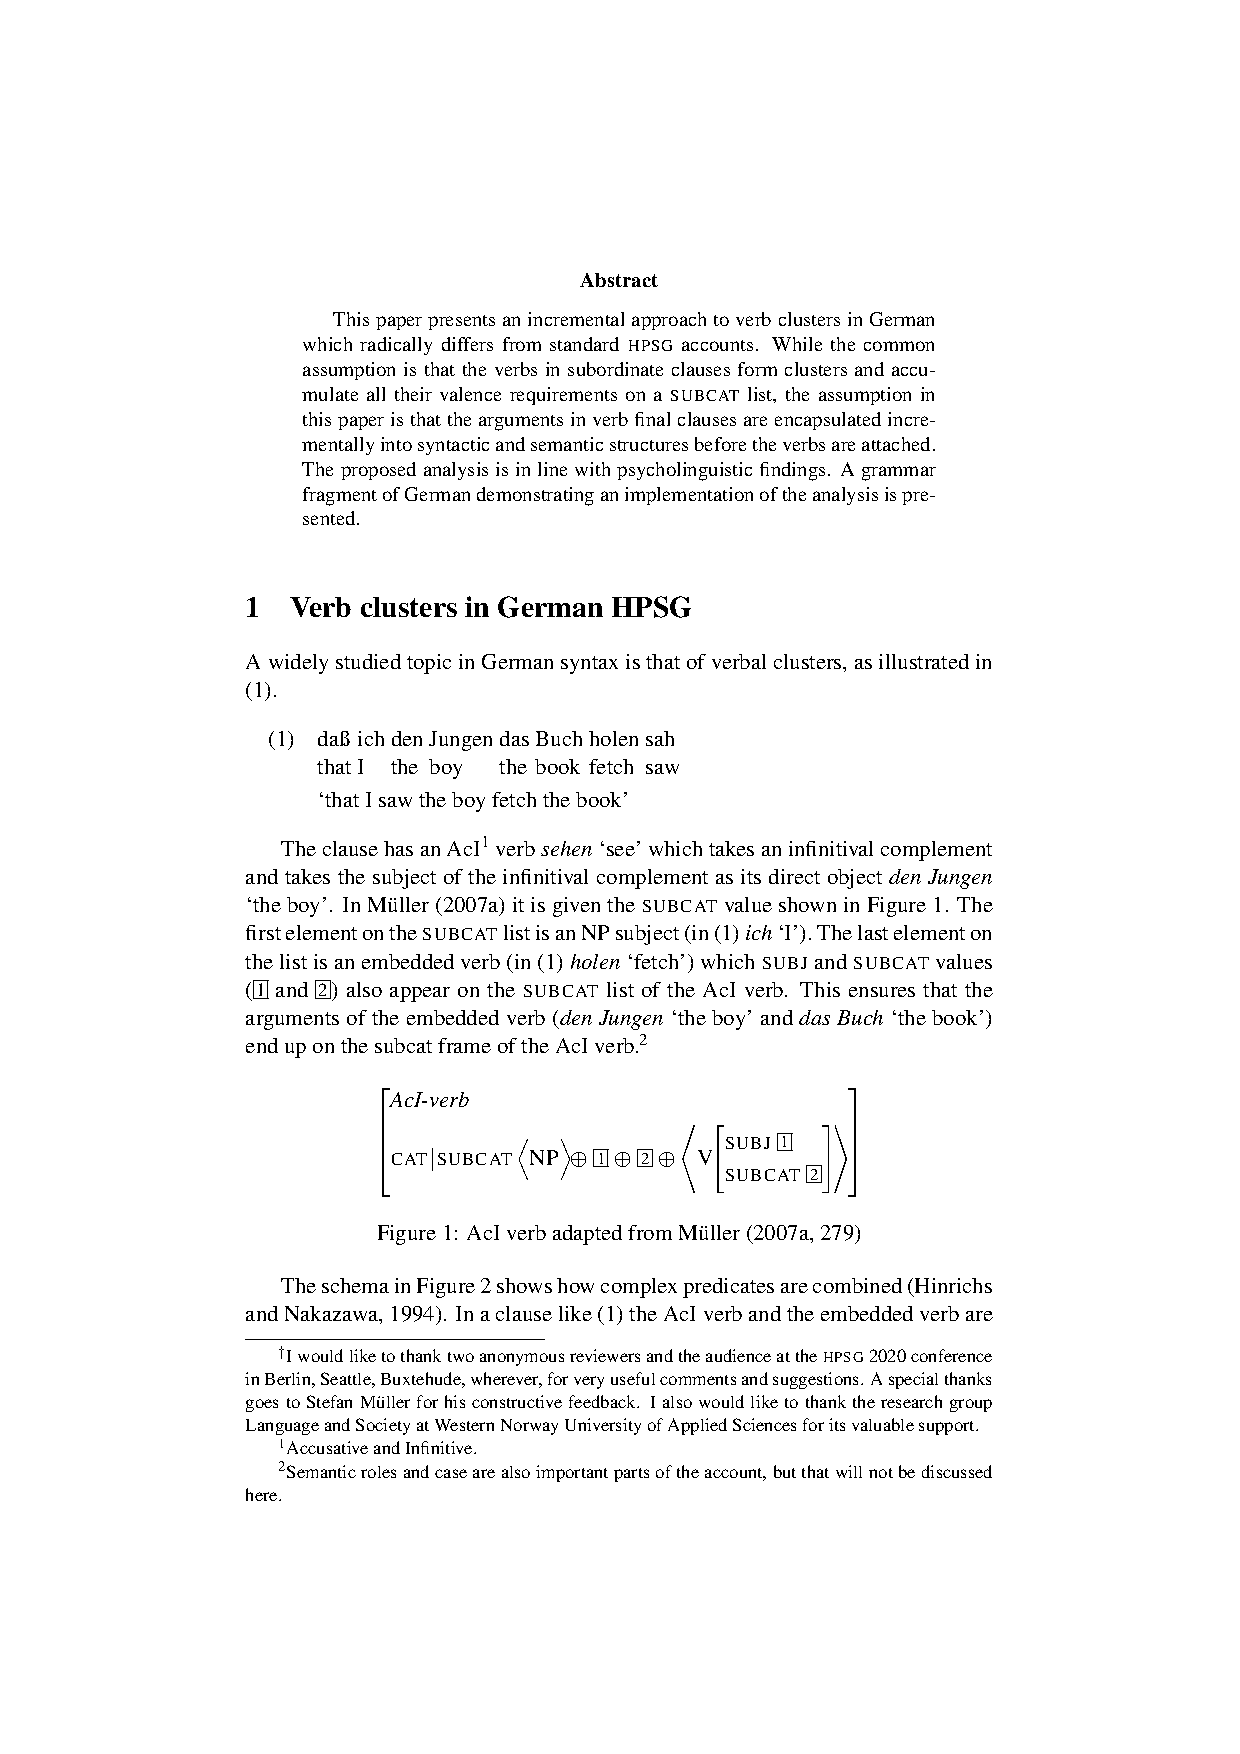
\includepdf[pages=-,pagecommand=\thispagestyle{plain}]{Includes/haugereid.pdf}
        \setcounter{page}{106}
        \phantomsection
        \addcontentsline{toc}{section}{Jean-Pierre Koenig, Karin Michelson: What does being a noun or a verb mean?}
\thispagestyle{empty}

\begin{center}
  {\huge\bfseries What does being a noun or a verb mean?\par}

  \bigskip

~\\
\begingroup
\setlength{\leftskip}{0pt plus 1fill}
\setlength{\rightskip}{0pt plus 1fill}
\setlength{\parindent}{0pt}
\setlength{\parfillskip}{0pt}
  \formatauthor{Jean-Pierre Koenig}{\begin{tabular}{@{}c@{}}Department of Linguistics and Center for Cognitive Science,
University at Buffalo\end{tabular}}
\formatauthor{Karin Michelson}{\begin{tabular}{@{}c@{}}Department of Linguistics and Center for Cognitive Science,
University at Buffalo\end{tabular}}

\par\endgroup

  \vspace*{8ex}

  Proceedings of the 27th International Conference on\par Head-Driven Phrase Structure Grammar

  \bigskip

  Online (Berlin/Seattle)

  \medskip

  Stefan  Müller, Anke Holler (Editors)

  \medskip

  2020

  \medskip

  CSLI Publications

  \medskip

  pages 106--126

  \medskip

  \url{http://csli-publications.stanford.edu/HPSG/2020}
\end{center}
\vfill

\noindent
Keywords: Oneida, Iroquoian, Parts of speech, Noun, Verb, Word Classes, Morphology


\vfill
\noindent
% APA Style
Koenig, Jean-Pierre, \& Michelson, Karin. 2020. What does being a noun or a verb mean? In Müller, Stefan, \& Holler, Anke (Eds.), \emph{{Proceedings of the 27th International Conference on Head-Driven Phrase Structure Grammar, Online (Berlin/Seattle)}}, 106--126. Stanford,
CA: CSLI Publications. \hfill\href{http://creativecommons.org/licenses/by/4.0/}{
\includegraphics[height=.75em]{Includes/ccby-eps-converted-to.pdf}}

\newpage
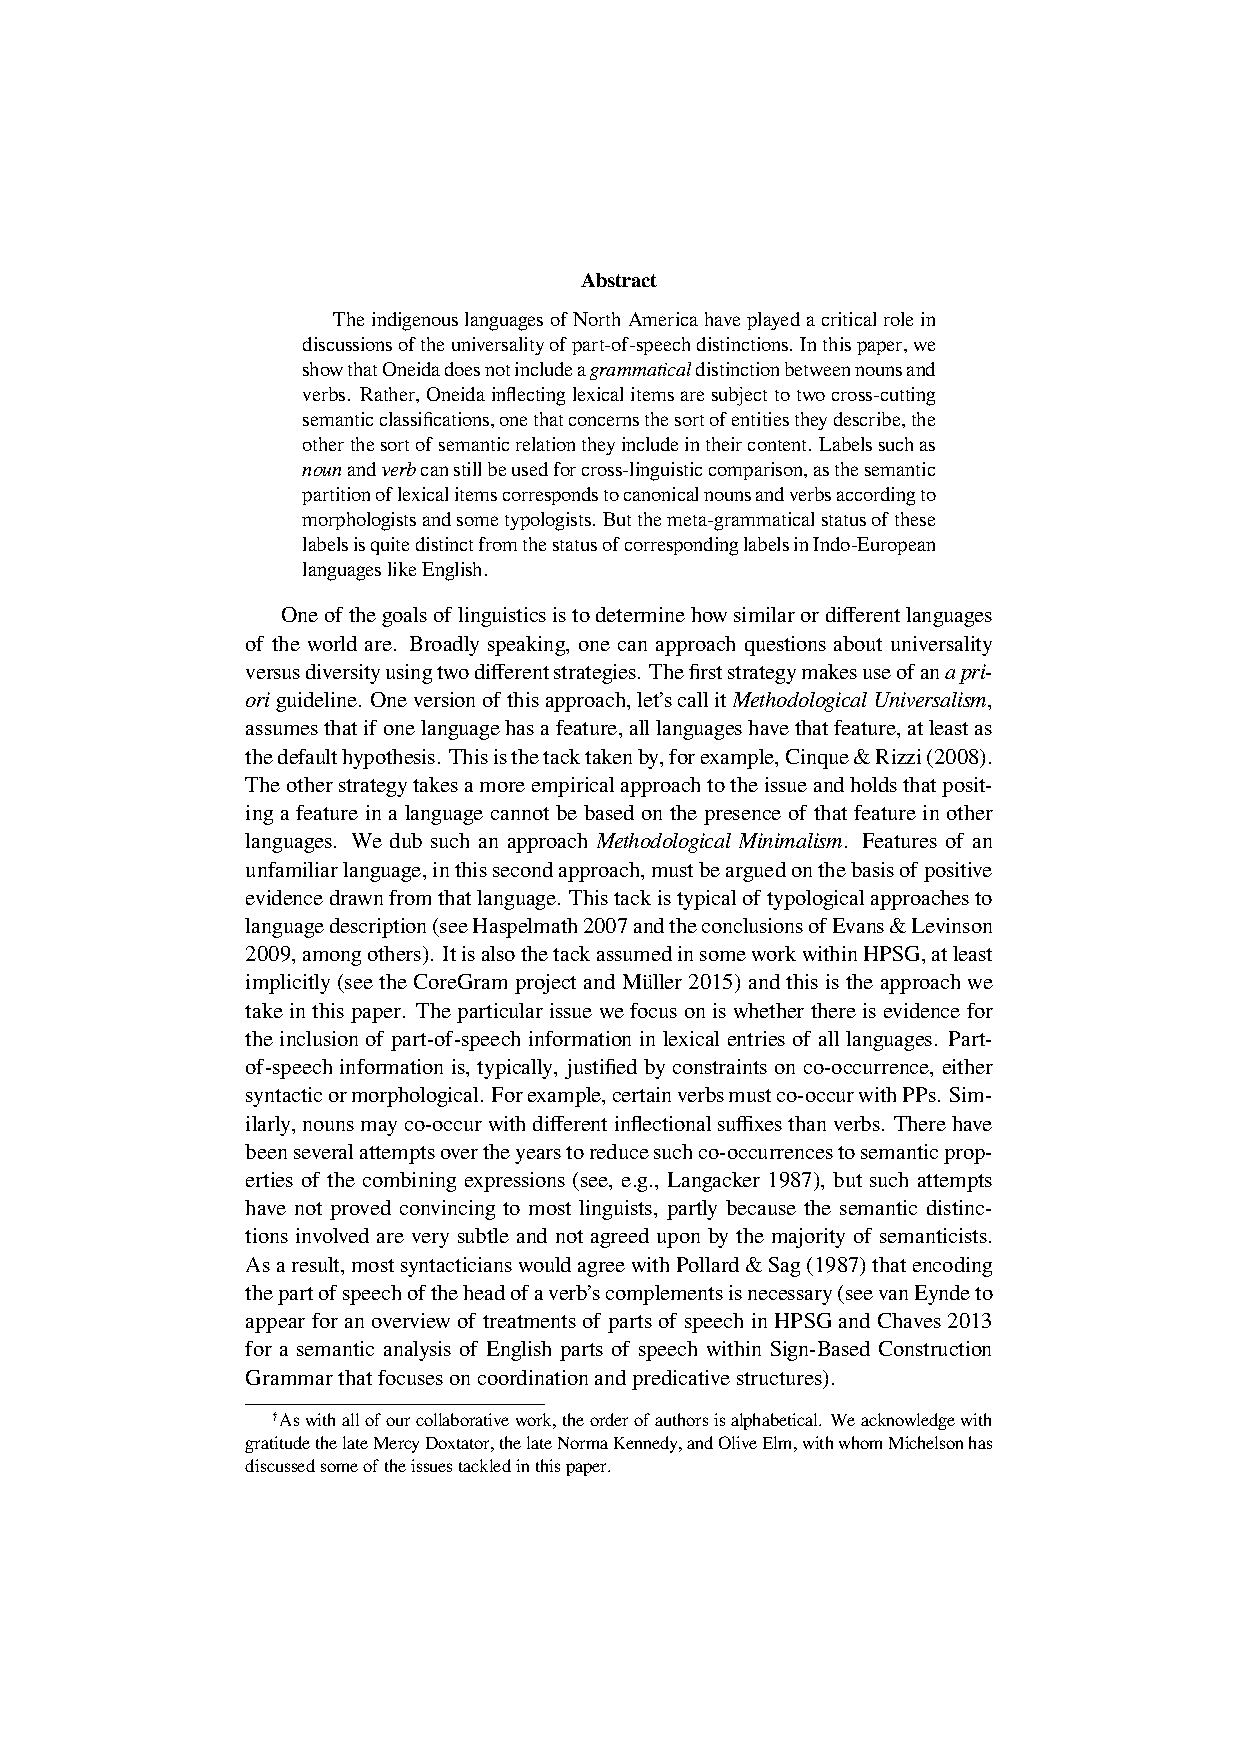
\includepdf[pages=-,pagecommand=\thispagestyle{plain}]{Includes/koenig-michelson.pdf}
        \setcounter{page}{127}
        \phantomsection
        \addcontentsline{toc}{section}{Frank Richter: Recursive adjectival modification in CLLRS}
\thispagestyle{empty}

\begin{center}
  {\huge\bfseries Recursive adjectival modification in CLLRS\par}

  \bigskip

~\\
\begingroup
\setlength{\leftskip}{0pt plus 1fill}
\setlength{\rightskip}{0pt plus 1fill}
\setlength{\parindent}{0pt}
\setlength{\parfillskip}{0pt}
  \formatauthor{Frank Richter}{\begin{tabular}{@{}c@{}}Goethe Universität Frankfurt am Main\end{tabular}}

\par\endgroup

  \vspace*{8ex}

  Proceedings of the 27th International Conference on\par Head-Driven Phrase Structure Grammar

  \bigskip

  Online (Berlin/Seattle)

  \medskip

  Stefan  Müller, Anke Holler (Editors)

  \medskip

  2020

  \medskip

  CSLI Publications

  \medskip

  pages 127--135

  \medskip

  \url{http://csli-publications.stanford.edu/HPSG/2020}
\end{center}
\vfill

\noindent
Keywords: HPSG,
semantics of modification, LRS, CLLRS


\vfill
\noindent
% APA Style
Richter, Frank. 2020. Recursive adjectival modification in CLLRS. In Müller, Stefan, \& Holler, Anke (Eds.), \emph{{Proceedings of the 27th International Conference on Head-Driven Phrase Structure Grammar, Online (Berlin/Seattle)}}, 127--135. Stanford,
CA: CSLI Publications. \hfill\href{http://creativecommons.org/licenses/by/4.0/}{
\includegraphics[height=.75em]{Includes/ccby-eps-converted-to.pdf}}

\newpage
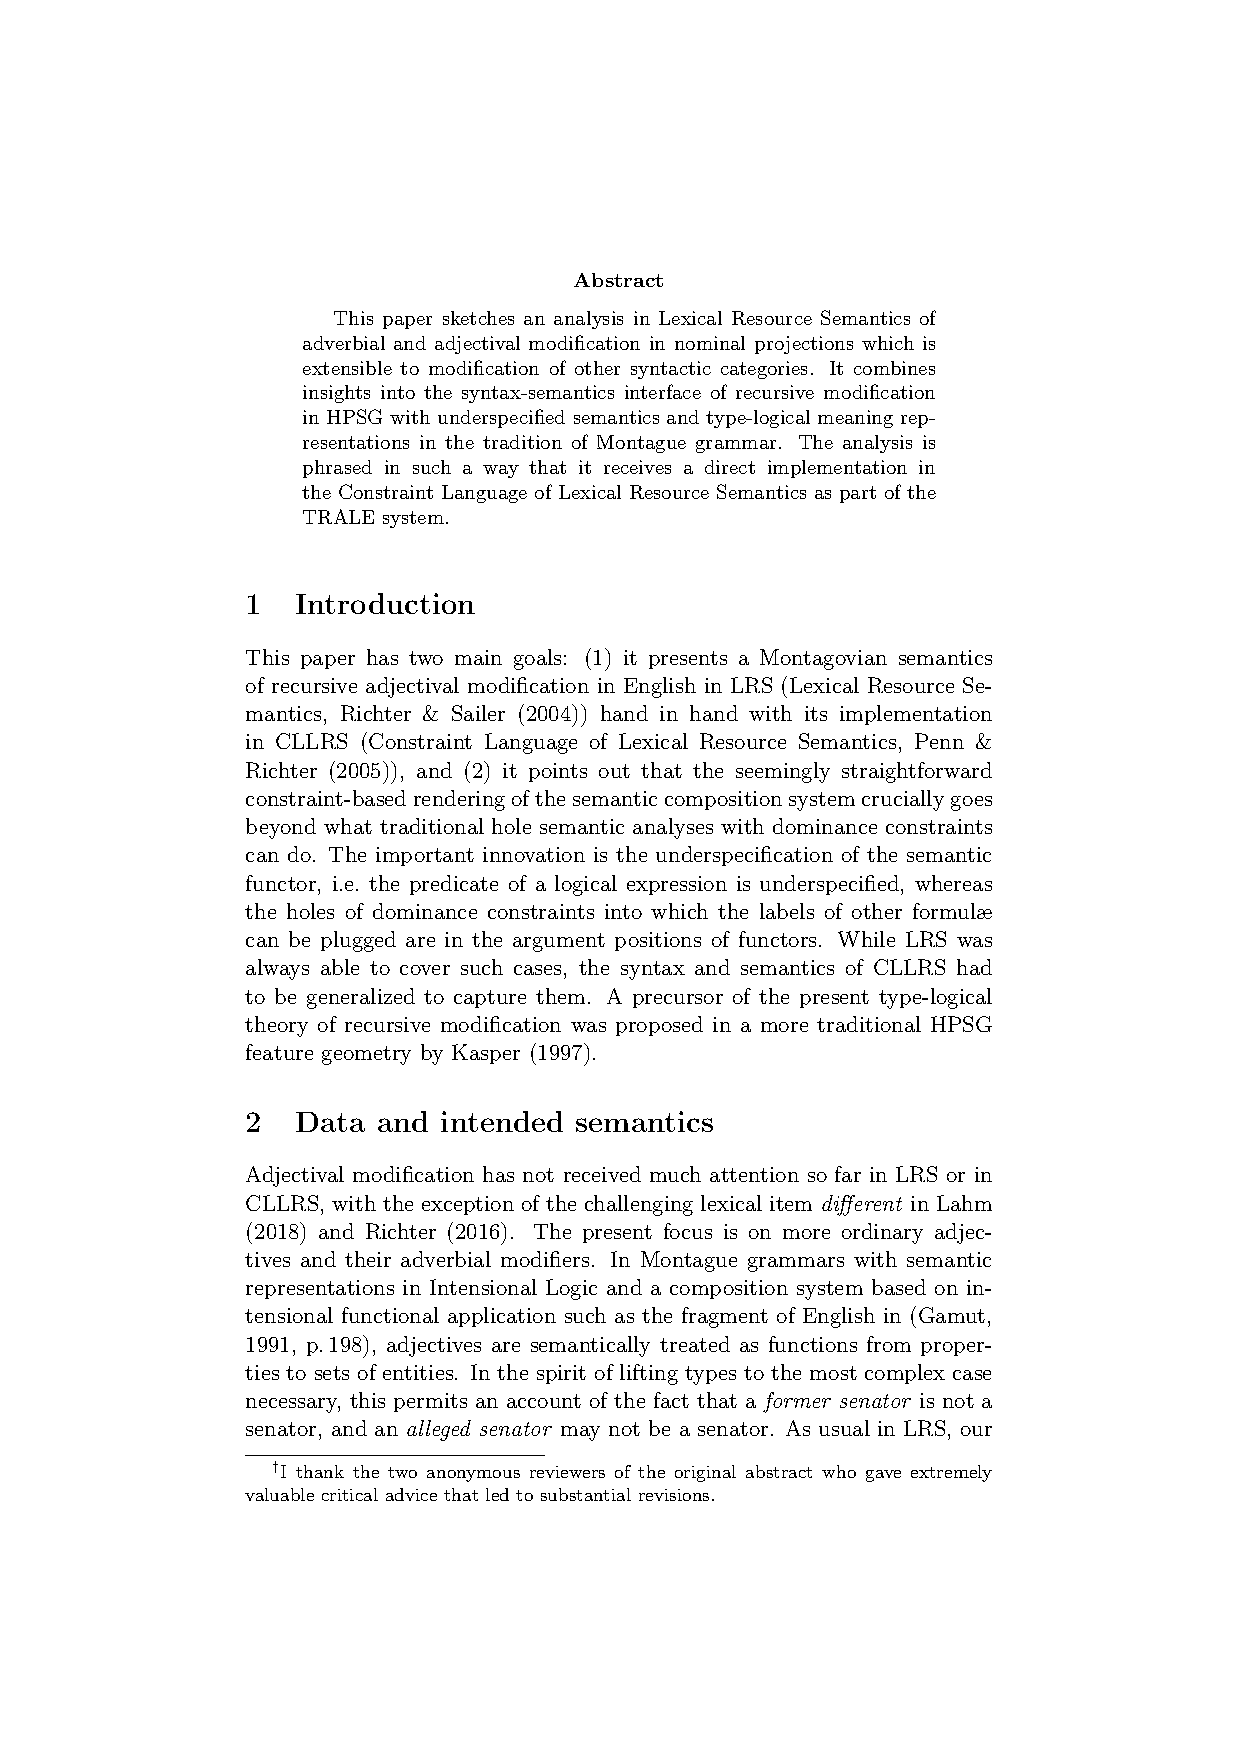
\includepdf[pages=-,pagecommand=\thispagestyle{plain}]{Includes/richter.pdf}
        \setcounter{page}{136}
        \phantomsection
        \addcontentsline{toc}{section}{Manfred Sailer, Annika D{\"o}rner: A
Smurf-based Approach to Placeholder Expressions}
\thispagestyle{empty}

\begin{center}
  {\huge\bfseries A
Smurf-based Approach to Placeholder Expressions\par}

  \bigskip

~\\
\begingroup
\setlength{\leftskip}{0pt plus 1fill}
\setlength{\rightskip}{0pt plus 1fill}
\setlength{\parindent}{0pt}
\setlength{\parfillskip}{0pt}
  \formatauthor{Manfred Sailer}{\begin{tabular}{@{}c@{}}Goethe-University Frankfurt a.M.\end{tabular}}
\formatauthor{Annika Dörner}{\begin{tabular}{@{}c@{}}University of Erfurt\end{tabular}}

\par\endgroup

  \vspace*{8ex}

  Proceedings of the 27th International Conference on\par Head-Driven Phrase Structure Grammar

  \bigskip

  Online (Berlin/Seattle)

  \medskip

  Stefan  Müller, Anke Holler (Editors)

  \medskip

  2020

  \medskip

  CSLI Publications

  \medskip

  pages 136--156

  \medskip

  \url{http://csli-publications.stanford.edu/HPSG/2020}
\end{center}
\vfill

\noindent
Keywords: German, HPSG, morphology, placeholder expression, smurfing


\vfill
\noindent
% APA Style
Sailer, Manfred, \& Dörner, Annika. 2020. A
Smurf-based Approach to Placeholder Expressions. In Müller, Stefan, \& Holler, Anke (Eds.), \emph{{Proceedings of the 27th International Conference on Head-Driven Phrase Structure Grammar, Online (Berlin/Seattle)}}, 136--156. Stanford,
CA: CSLI Publications. \hfill\href{http://creativecommons.org/licenses/by/4.0/}{
\includegraphics[height=.75em]{Includes/ccby-eps-converted-to.pdf}}

\newpage
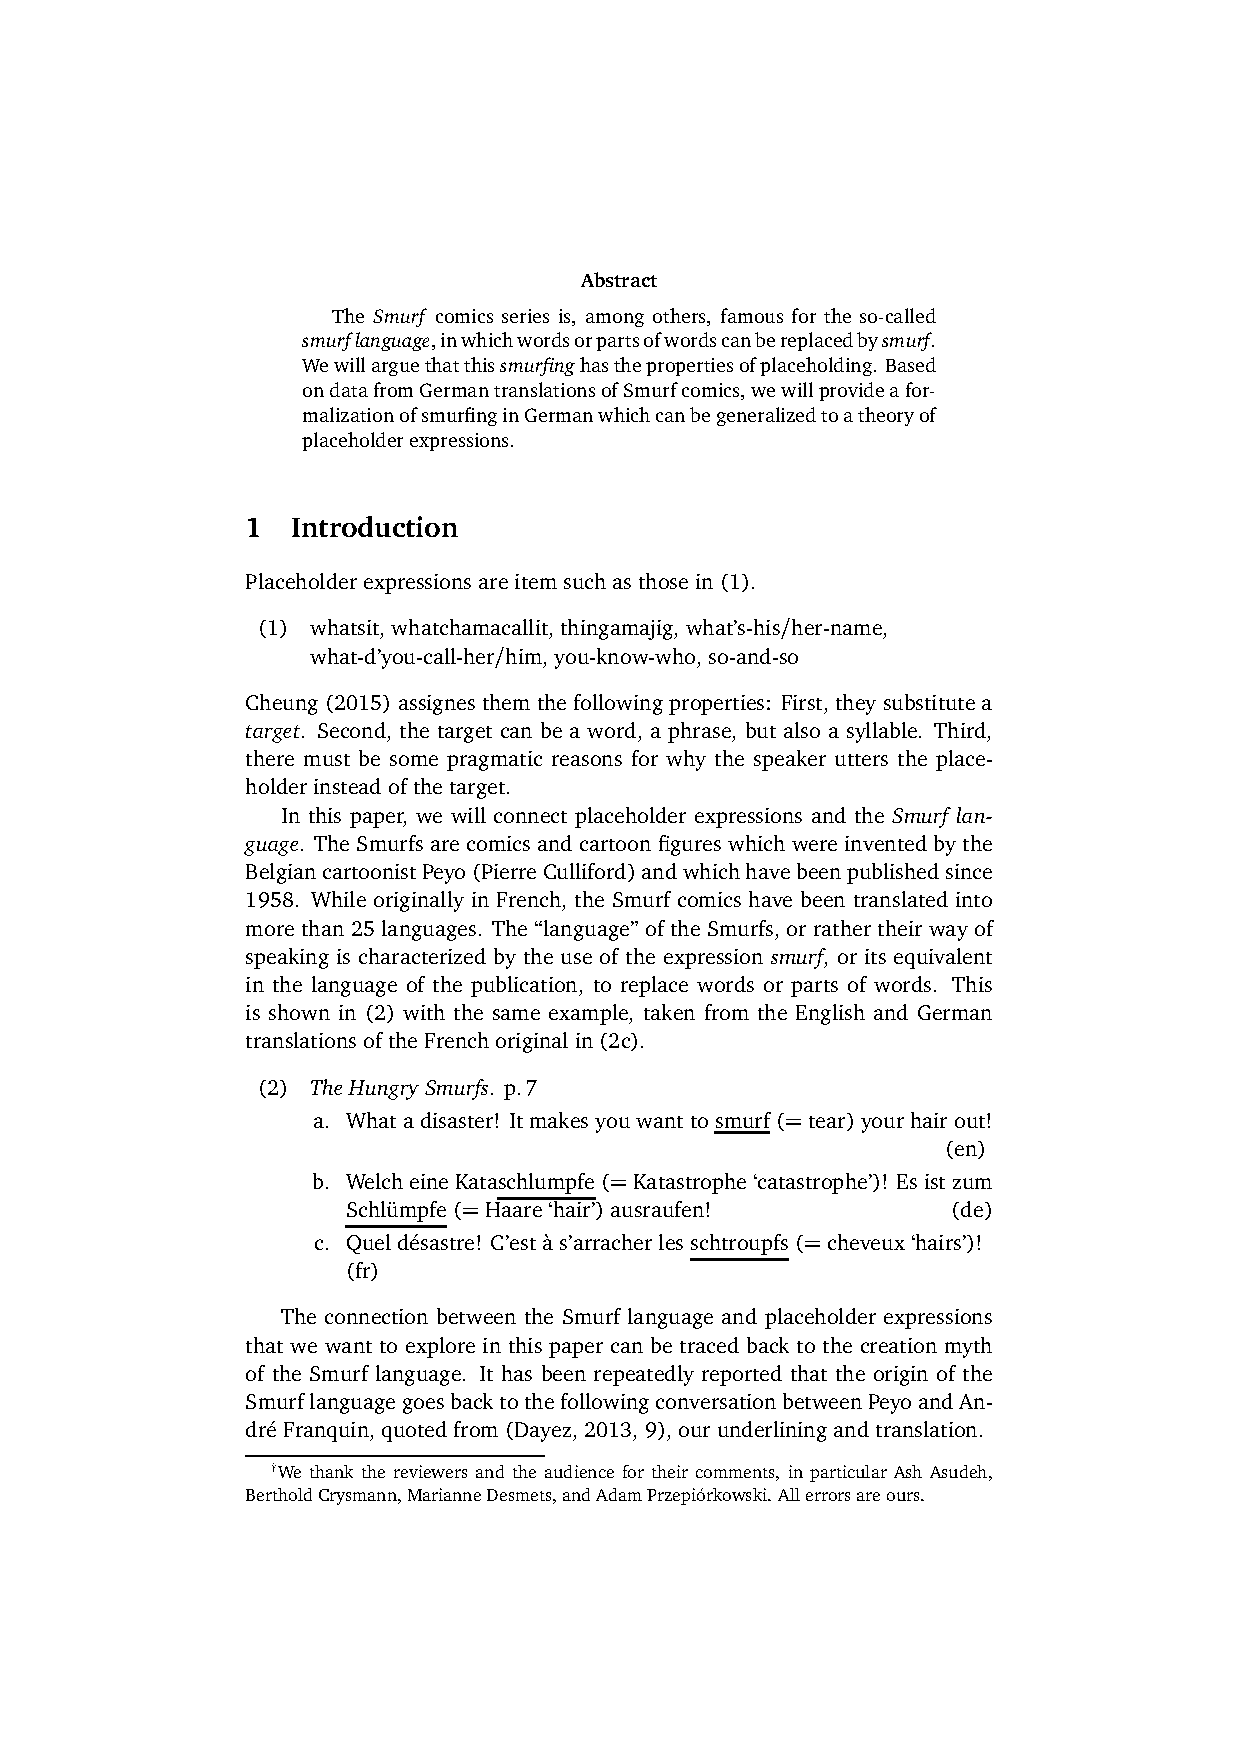
\includepdf[pages=-,pagecommand=\thispagestyle{plain}]{Includes/sailer-doerner.pdf}
        \setcounter{page}{157}
        \phantomsection
        \addcontentsline{toc}{section}{Olga Zamaraeva, Guy Emerson: Multiple Question Fronting without Relational Constraints:  An Analysis of Russian as a Basis for Cross-Linguistic Modeling}
\thispagestyle{empty}

\begin{center}
  {\huge\bfseries Multiple Question Fronting without Relational Constraints:  An Analysis of Russian as a Basis for Cross-Linguistic Modeling\par}

  \bigskip

~\\
\begingroup
\setlength{\leftskip}{0pt plus 1fill}
\setlength{\rightskip}{0pt plus 1fill}
\setlength{\parindent}{0pt}
\setlength{\parfillskip}{0pt}
  \formatauthor{Olga Zamaraeva}{\begin{tabular}{@{}c@{}}University of Washington\end{tabular}}
\formatauthor{Guy Emerson}{\begin{tabular}{@{}c@{}}University of Cambridge\end{tabular}}

\par\endgroup

  \vspace*{8ex}

  Proceedings of the 27th International Conference on\par Head-Driven Phrase Structure Grammar

  \bigskip

  Online (Berlin/Seattle)

  \medskip

  Stefan  Müller, Anke Holler (Editors)

  \medskip

  2020

  \medskip

  CSLI Publications

  \medskip

  pages 157--177

  \medskip

  \url{http://csli-publications.stanford.edu/HPSG/2020}
\end{center}
\vfill

\noindent
Keywords: HPSG, interrogatives, wh-questions, Russian, Grammar Matrix, multiple fronting, DELPH-IN, difference lists, append lists, lists


\vfill
\noindent
% APA Style
Zamaraeva, Olga, \& Emerson, Guy. 2020. Multiple Question Fronting without Relational Constraints:  An Analysis of Russian as a Basis for Cross-Linguistic Modeling. In Müller, Stefan, \& Holler, Anke (Eds.), \emph{{Proceedings of the 27th International Conference on Head-Driven Phrase Structure Grammar, Online (Berlin/Seattle)}}, 157--177. Stanford,
CA: CSLI Publications. \hfill\href{http://creativecommons.org/licenses/by/4.0/}{
\includegraphics[height=.75em]{Includes/ccby-eps-converted-to.pdf}}

\newpage
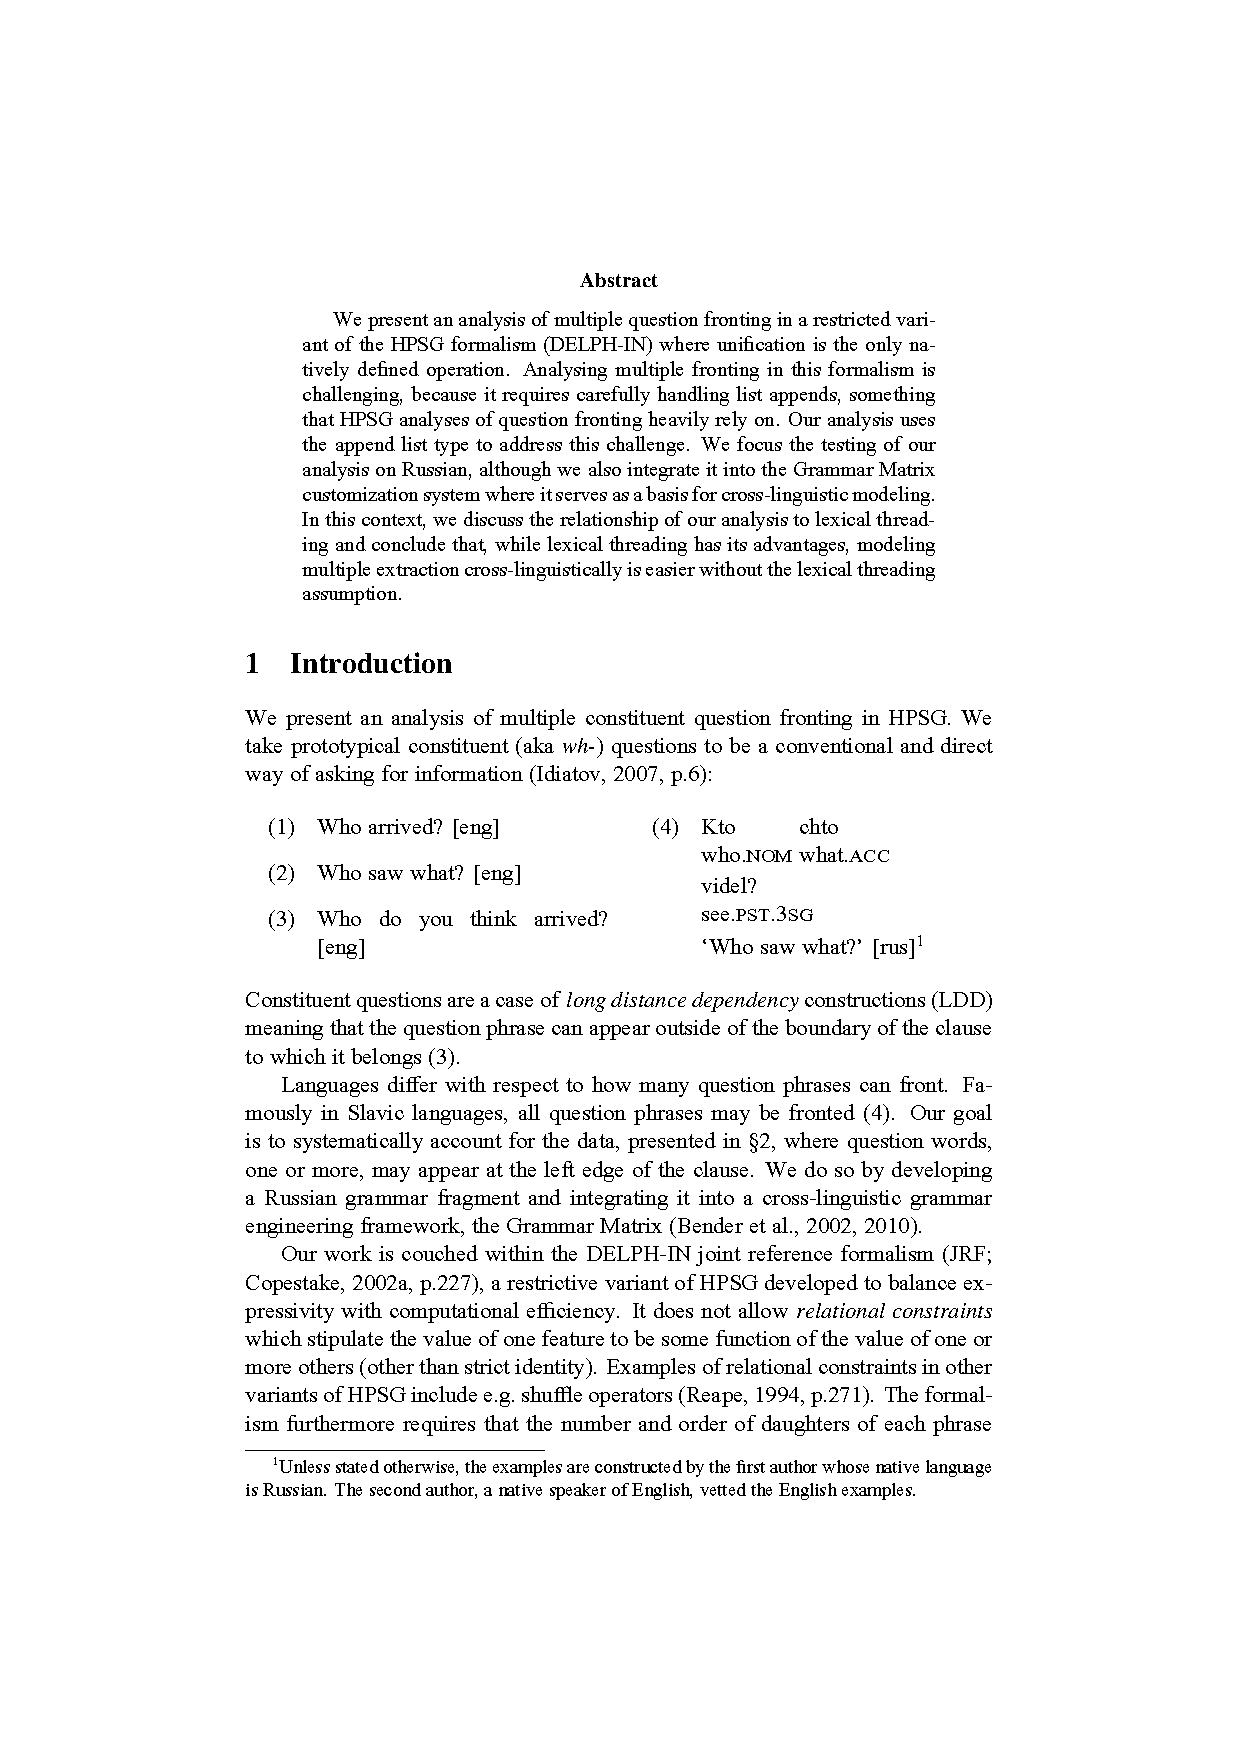
\includepdf[pages=-,pagecommand=\thispagestyle{plain}]{Includes/zamaraeva-emerson.pdf}
\end{document}
